\section{Cubedate: Standard Security for Continuous Deployment of Low-power CubeSat Software}
\label{sec:low-power-orbital-communication-arch}


The minimal security guarantees that we aim for are authenticity and integrity of software udpates, during the lifetime of the satellite mission.
These guarantees must remain valid end-to-end, all the way from the hosted payload software maintainer to the payload hosted in orbit on the CubeSat.
The basic process we use for securing authenticity and integrity of software udpates is decomposed in six phases shown \autoref{fig:phases}. 

\subsection{Basic Software Life-cycle Phases}

During a preliminary, pre-flight phase (\textit{Phase 0}) the authorized maintainer for the CubeSat-hosted payload
produces and flashes the payload with commissioning material:
a bootloader, the initial firmware, and authorized crypto material (a public key, and a crypographically strong hash function).
Once the hosted payload is commissioned it can be sent to the CubeSat operator of installation in the CubeSat.


Once the CubeSat in orbit, the hosted payload maintainer can trigger iterations through cycles of Phases 1-5, whereby
the authorized maintainer can build a new software update (\textit{Phase 1}), hash the update
and sign the hash (\textit{Phase 2}) then push a network transfer (PUT) towards the hosted payload via the ground station and the OBC (\textit{Phase 3.1}). The next time it wakes up, the hosted payload can
then ping and fetch (GET) the update from the OBC (\textit{Phase 3.2}), proceed to verify the signature and the hash (\textit{Phase 4}),
and upon successful verification, install/boot the new software (\textit{Phase 5}), otherwise the update is dropped.

\begin{figure}[t]
    \centering
    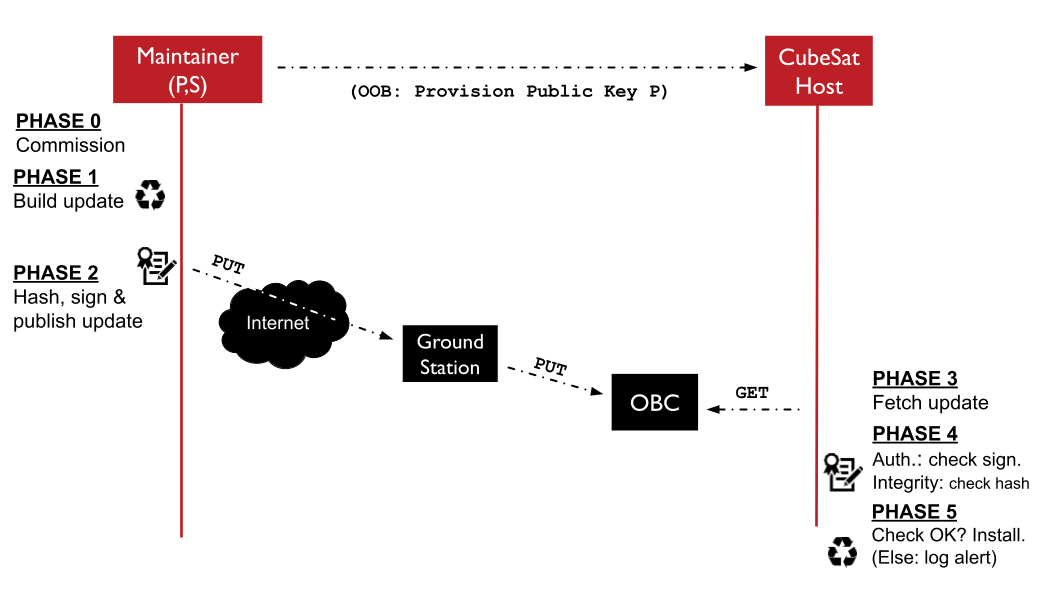
\includegraphics[width=0.5\textwidth]{Figures/CubeSat-Payload-update.png}
    \caption{CubeSat hosted payload secure software update process.}
    \label{fig:phases}
\end{figure}

\subsection{Supporting Network Transport Heterogeneity}
This aspect concerns both \textit{Phase 3.1} and \textit{Phase 3.2} in \autoref{fig:phases}. 

First of all, software updates may be transported over a wide variety of network segments.
\begin{itemize}
\item {\bf Developer-Groundstation segment}: via wired Internet, USB key upload...
\item {\bf Groundstation-CubeSat segment}: via radio links such as UHF, LoRa...
\item {\bf Intra-CubeSat segment}: via bus communication such as CAN/CSP, SPI...
\end{itemize}

Second, paths across the network may vary in complexity.
In the simplest case (typical CubeSat use-case) the end-to-end network path covers only the segment from ground station to the OBC.
In more complex cases involving hosted payloads, not only
must the end-to-end path traverse heterogeneous network segments,
but also: this path may never exist end-to-end at any point in time.
This Delay-tolerant network characteristic is due to power-off periods imposed on CubeSat hosted payloads, 
combined with orbiting CubeSat being out-of-range most of the time via radio w.r.t. available ground stations.
Hence, while in transit across the network, software update data may have to be temporarily cached at some intermediate node along the path.

To cope with this wide variety of scenarios, different solutions may be used at the network, transport and application layers. \todoEB{Add here some short text about what ThingSat does, also hint at exotic things such as ICN?}. 


However, Cubedate does not specify the use of any particular approach at the network, transport and application layers to enable the delivery of software updates across the network.
Cubedate only aims to guarantee end-to-end security properties for the software update binaries delivered over the network.

\subsection{Supporting Updated Software Heterogeneity}
This aspect concerns both \textit{Phase 1} and \textit{Phase 5} in \autoref{fig:phases}. 
Software that must be updated may be of various nature, and size.
(1 )Firmware updates, (2) Mission/configuration files, (3) things like Femto-containers?.

\subsection{Low-power Standardized End-to-End Security}

\todoEB{Describe and motivate here use of of SUIT metadata.}

Using Cubedate and the SUIT standard, software updates for payload hosted on CubeSats mitigate attacks including:

\begin{itemize}
\item {\bf Tampered Software Update Attacks –} An attacker may try to update the IoT device with a modified and intentionally flawed software image. To counter this threat, Cubedate uses digital signatures on a hash of the image binary and the metadata to ensure integrity of both the firmware and its metadata.

\item {\bf Unauthorized Software Update Attacks –} An unauthorized party may attempt to update the IoT device with modified image. Using digital signatures and public key cryptography, Cubedate ensures, that only the authorized maintainer (holding the authorized private key) will be able to update de device.
\end{itemize}

Going beyond simple authenticity and integrity guarantees for software updates delivered over the network, using Cubedate also mitigates other attacks including:
\begin{itemize}
\item {\bf Software Update Replay Attacks –} An attacker may try to replay a valid, but old (known-to-be-flawed) software. This threat is mitigated by using a sequence number. Cubedate uses a sequence number, which is increased with every new software update.

\item {\bf Software Update Mismatch Attacks –} An attacker may try replaying a software update that is authentic, but for an incompatible device. Cubedate includes device-specific conditions, which can be verified before installing a software binary, thereby preventing the device from attempting to use an incompatible software image.
\end{itemize}

\iffalse

\paragraph*{communication protocols}
\paragraph*{software/firmware updates}
\paragraph*{software/configuration updates requirements}

\subsection{Architecture}
\subsubsection{OS}: RIOT
\subsubsection{Network Stack}: COAP/LibCSP/CAN
\subsubsection{Mission Workflow}: mission files
\subsubsection{DevOps Workflow}: SUIT + containers
\paragraph*{SUIT}
\paragraph*{Containerization}
\fi
